\chapter{Testes do \textit{Clean Pool Robot}} \label{ch:tests-robot}
\section{Teste de Vedação - Persilox}
O teste do Persilox® teve por objetivo testar a eficácia do produto de vedação escolhido. Para tanto foi feito com o uso de um cabo, recipiente cilíndrico de plástico, balde com água e papel toalha.

No recipiente de plástico foi feito um furo, na sua lateral, do diâmetro do fio. Foi colocado o fio no furo e a vedado com o Persilox®. Depois de 10 minutos, a cola já estava seca, então colocou-se o papel toalha dentro do recipiente de plástico e mergulhou o mesmo no balde com água até que o fluido cobrisse a entrada do fio. Após um período retirou-se o recipiente da água e verificou-se que o papel toalha inserido no mesmo estava seco, além de visivelmente não haver a presença de umidade no interior do recipiente.

\section{Testes do Protótipo}
O teste do protótipo teve como objetivo a validação do  sistema de locomoção, composto pela união da base do robô com as rodas, a bomba e a fonte de tensão externa. O teste realizado pode ser dividido em duas partes: na parte I, o objetivo específico foi validar o sistema de vedação da alimentação Fonte-Bomba dentro d’água, e a  parte II o objetivo específico foi verificar se o conjunto conseguia se locomover dentro d’água somente com o jato da propulsão da bomba.

\subsection{Parte I : sistema de vedação da alimentação Fonte-Bomba}
Para a Parte I os fios de saída de alimentação da fonte, 12 V e entrada da bomba foram conectados com uma tomada macho e femêa, o que possibilitou a união de ambos. Esse ponto de união da Fonte-Bomba dista da posição da bomba, aproximadamente, um metro o que implica em imersão da conexão em água. A metodologia consistiu em realizar dois furos no recipiente, um em cada extremidade, passar a fiação e em seguida instalar as partes da tomada (macho e femêa), ao fechar os conectores o conjunto foi vedado com o Persilox® e em seguida, coberto com fita isolante. O conjunto foi colocado na piscina e, por constatação visual, observou-se que o conjunto ainda apresentava alguns pontos não vedados, pois começou a entrar água no recipiente. Como solução ao impasse, o recipiente e conector serão alterado para a melhor segurança da parte elétrica. A Figura \ref{fig:isolation} apresenta o item testado.
\par
\begin{figure}[h]
  \centering
  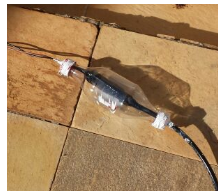
\includegraphics[width=0.6\textwidth]{figures/isolation.png}
  \caption{Isolação do sistema Bomba-Fonte.}
  \label{fig:isolation}
\end{figure}
\FloatBarrier
\par

\subsection{Parte II : sistema de Locomoção}
A Parte II do teste consistiu em anexar a bomba de sucção juntamente a base da estrutura a fim de se avaliar a movimentação do robô através da propulsão dentro da piscina. Admitindo uma coluna d’água de aproximadamente 1.65 metros, com o teste de movimentação era esperado de acordo com os cálculos uma velocidade de deslocamento de entorno 15 cm/s, admitindo uma vazão nominal sem perdas gerado pela bomba de sucção e o peso total do sistema (conjunto base-bomba) cerca de 4 Kg. Após o teste foi possível avaliar que o teste de movimentação através da propulsão apresentou uma velocidade de aproximadamente 15 cm/s. Seguido deste, foi definido realizar novamente o teste, com intuito de avaliar a movimentação com uma carga adicional de 5 Kg, a fim de analisar a possível carga completa do robô.

\par
\begin{figure}[h]
  \centering
  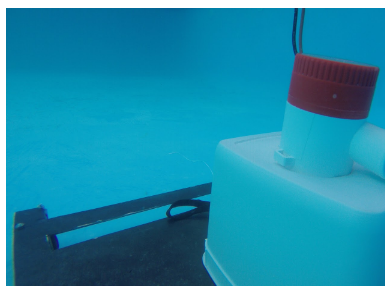
\includegraphics[width=0.6\textwidth]{figures/test.png}
  \caption{Teste de movimentação Robô.}
  \label{fig:test}
\end{figure}
\par
